\section{Results}

As described above, the proportion of each gender getting funded will be displayed first; the following will show the detailed results comparing different classifications and universities across time. The calculated p-value of hypothesis testing will also be indicated.

\subsection{Total funding across time}

\begin{figure}[H]
    \centering
    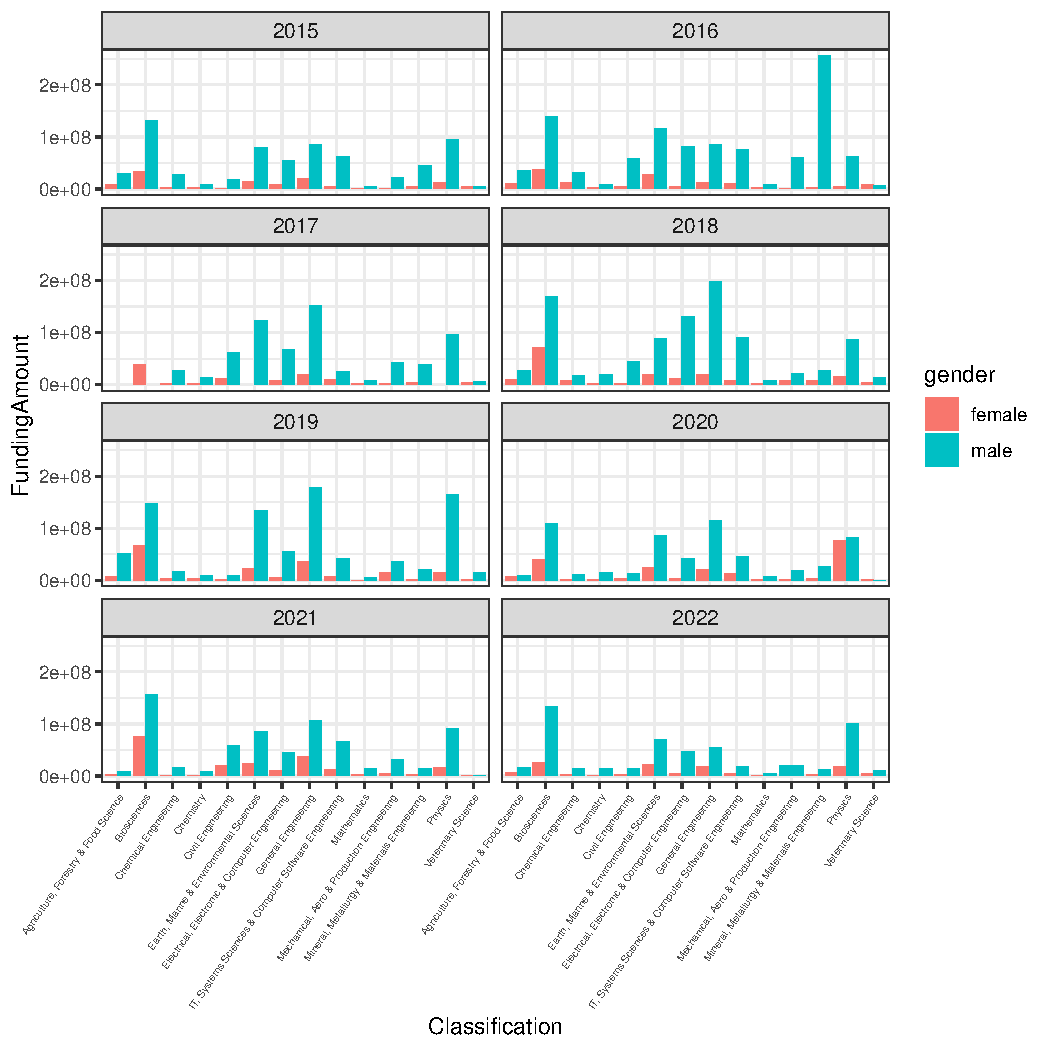
\includegraphics[width = 1\textwidth]{funding_all.pdf}
    \caption{The plot shows the total research funding allocated to each gender during the period measured in GBP.}
\end{figure}

From this result, a great gender gap is seen. The graph indicates that the gender gap in recent years is smaller compared to the first three years when the funding amount for females almost cannot be seen compared to males. The Biosciences field has the greatest amount of funding for females across time, except in 2020, when the gender gap in Physics is the smallest. Despite an emerging trend towards bridging the gender gap, the progress is subtle, and the overall scenario remains concerning.\\
\\
\noindent For the robustness of our result, a two-sample t-test is conducted for the number of funded males and females in different years. According to the result of the two-sample t-test, the t-statistic, representing the difference between the mean of the two data groups, is approximately 8.40; the p-value is 6.918e-14, much smaller than a significance level of 0.05. This result provides strong evidence to reject the null hypothesis, indicating a significant difference between the mean of research funding allocated to males and females from 2015 to 2022.

\subsection{Temporal trends comparison}

This subsection will display the comparison results for the temporal trends across the various STEM categories and institutions. The proportion of males and females getting funded will be shown in a time-series form. At the same time, I will show the ranking of the degree of bias across time to find the source of the disparity.

\subsubsection{Comparison among classifications}
\begin{figure}
    \centering
    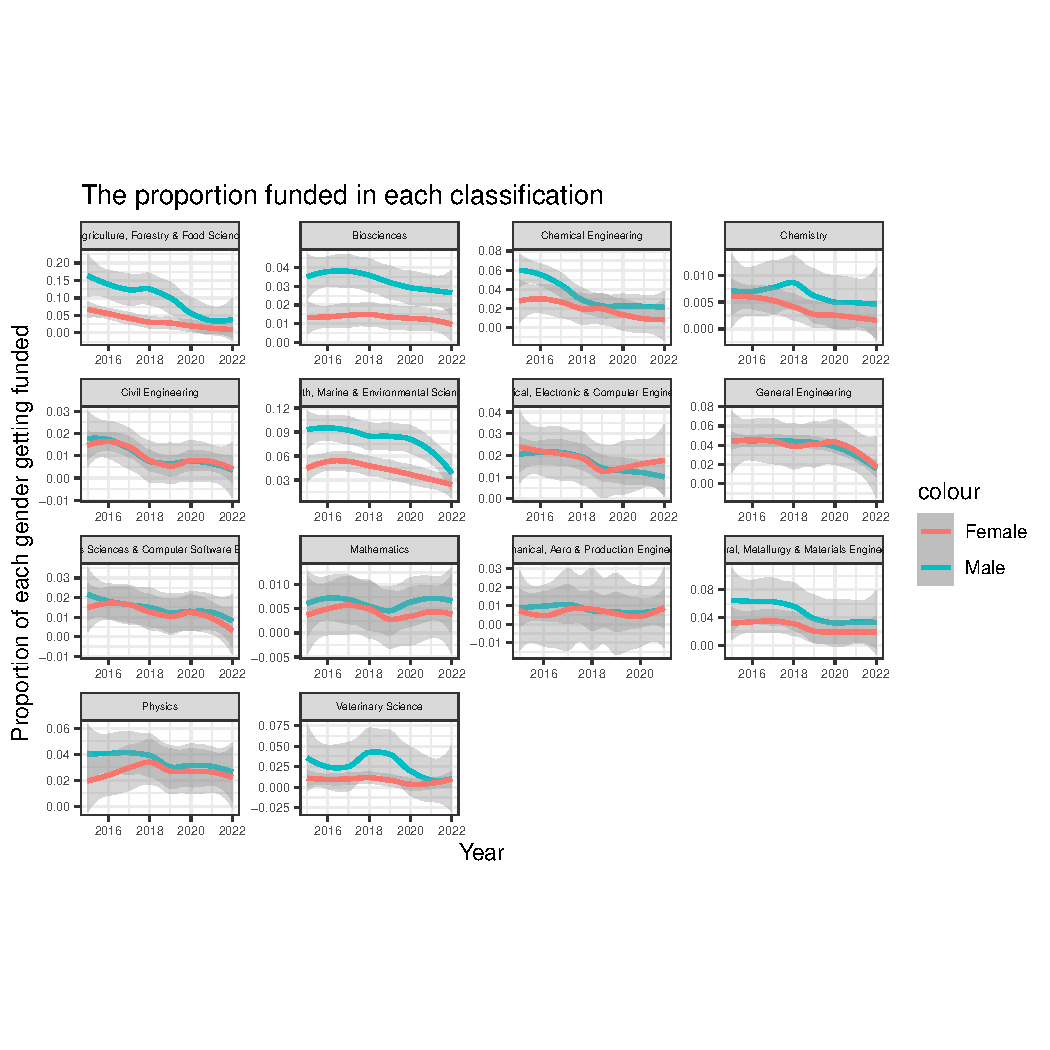
\includegraphics{plots_classification.pdf}
    \caption{This figure shows the general trend of funded proportion in each classification across time. In this result, the proportion of each gender is used, calculated by dividing the funded males or females by the total number of HESA staff in each gender. The grey area represents the 0.95 confidence interval - a narrower band usually indicates a more precise result.}
\end{figure}
\begin{figure}
	\centering
	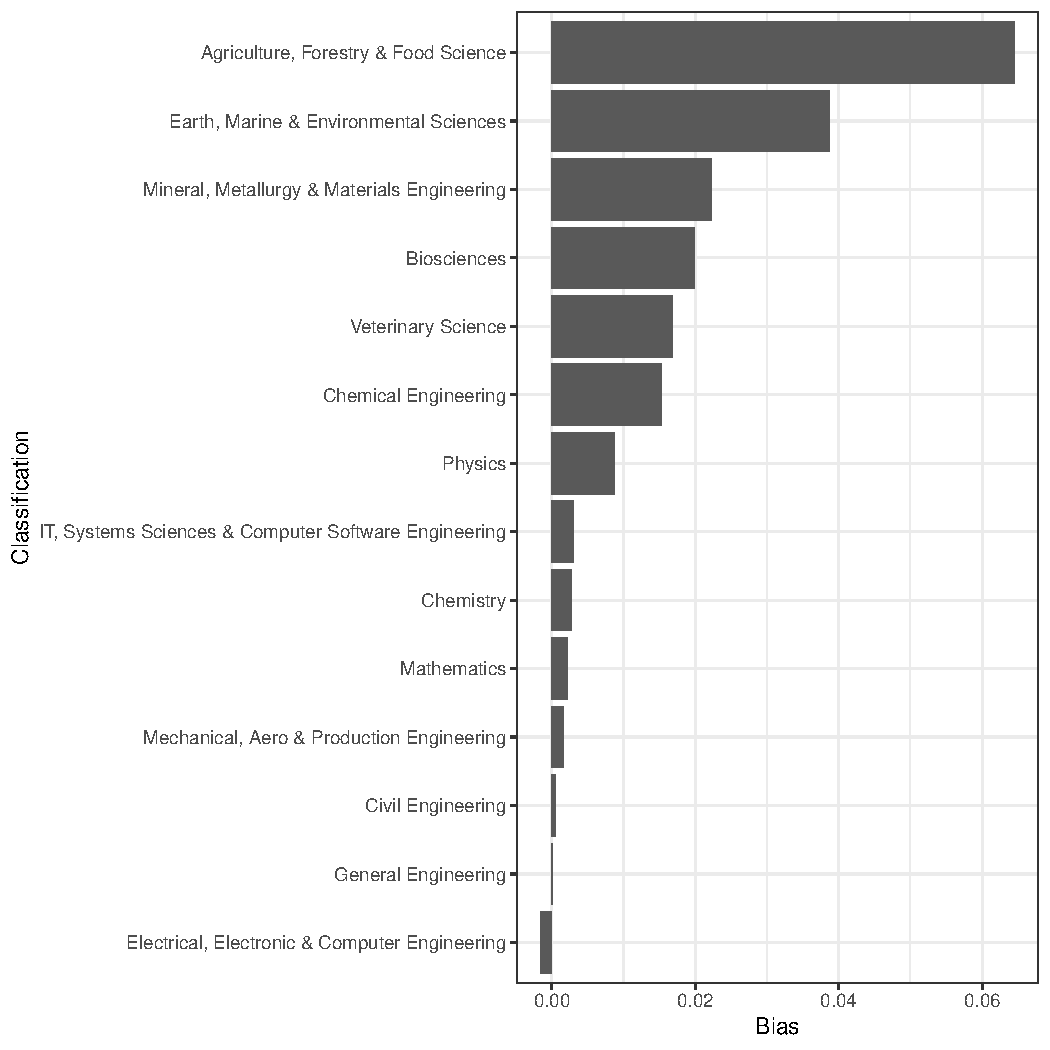
\includegraphics[width=0.8\textwidth]{rank_class.pdf}
	\caption{This figure shows the ranking of the extent of gender bias in each classification across time. For the bias degree, I calculated the total number of funded males or females from 2015 to 2022, divided by the total number of HESA staff in the corresponding gender during the period. Then, the difference of the ratios for males and females is conducted and is reordered depending on the degree of biases - the upper represents the classification with greater gender bias.}
\end{figure}

\noindent As displayed in Figures 2 and 3, the results show a great gender gap in the research funding of Biosciences, where the gap almost persists; though the extent of gender bias overall is the greatest in Agriculture, Forestry \& Food Science, the disparity has been considered diminished in the latest years. By contrast, there are several categories where the proportion of both genders is nearly the same over time, including General Engineering, Civil Engineering, and IT, Systems Sciences \& Computer Software Engineering. In most classifications, there is an encouraging trend indicating a reduction in the gap between males and females. An exception would be Chemistry, where the gender gap increased over time. An interesting observation is that in the field of Electrical, Electronic \& Computer Engineering, the proportion of funded females even exceeded that of males in recent years. 

\subsubsection{Comparison among universities}
As one of the primary criteria of the research application, university ranking would be an important factor that may affect funding fairness. The ratio of funded researchers in different universities is displayed in Figures 4 and 5, where each colour represents a classification, and the scales for each subplot were set to be the same; only the universities with sufficient funding data are selected for the comparison.
\begin{figure}
\caption{This figure shows the comparison among different universities. The results of 65 universities were generated in my study; however, only 12 of them were selected. The reason is that some of the universities have little funding data, therefore only the universities with the most number of results displayed are selected for analysis.}
\begin{tikzpicture}
    \node(img){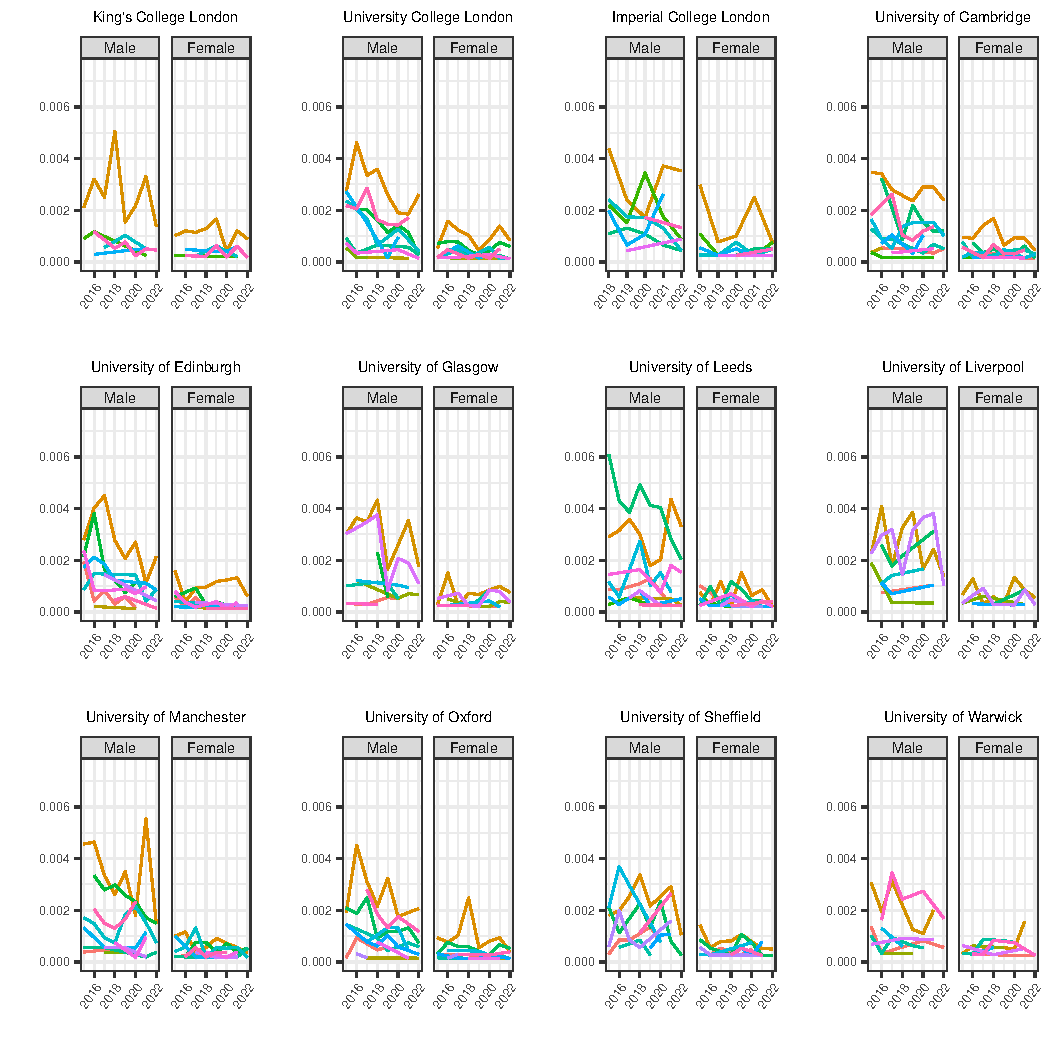
\includegraphics[page=1, scale=0.8]{uni_selected.pdf}};
    \node[below=of img, node distance=0cm, yshift=1cm,font=\color{black}\large] {Year};
    \node[left=of img, node distance=0cm, rotate=90, anchor=center,yshift=-0.7cm,font=\color{black}\large] {Ratio of each gender getting funded};
\end{tikzpicture}
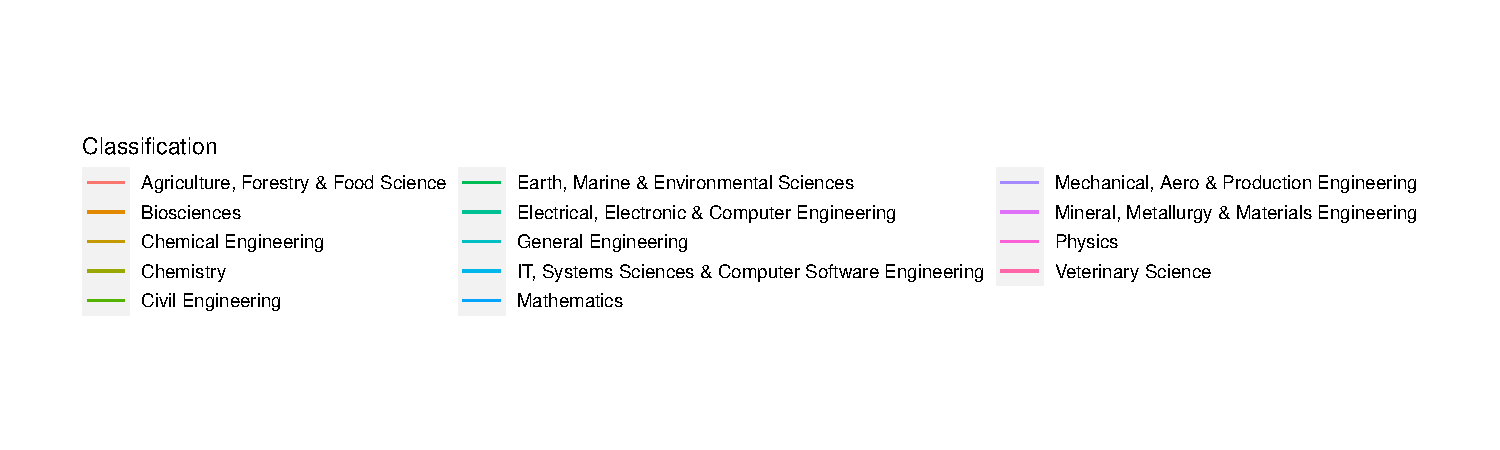
\includegraphics[page=1, scale=0.6]{legend.pdf}
\end{figure}

\begin{figure}
	\centering
	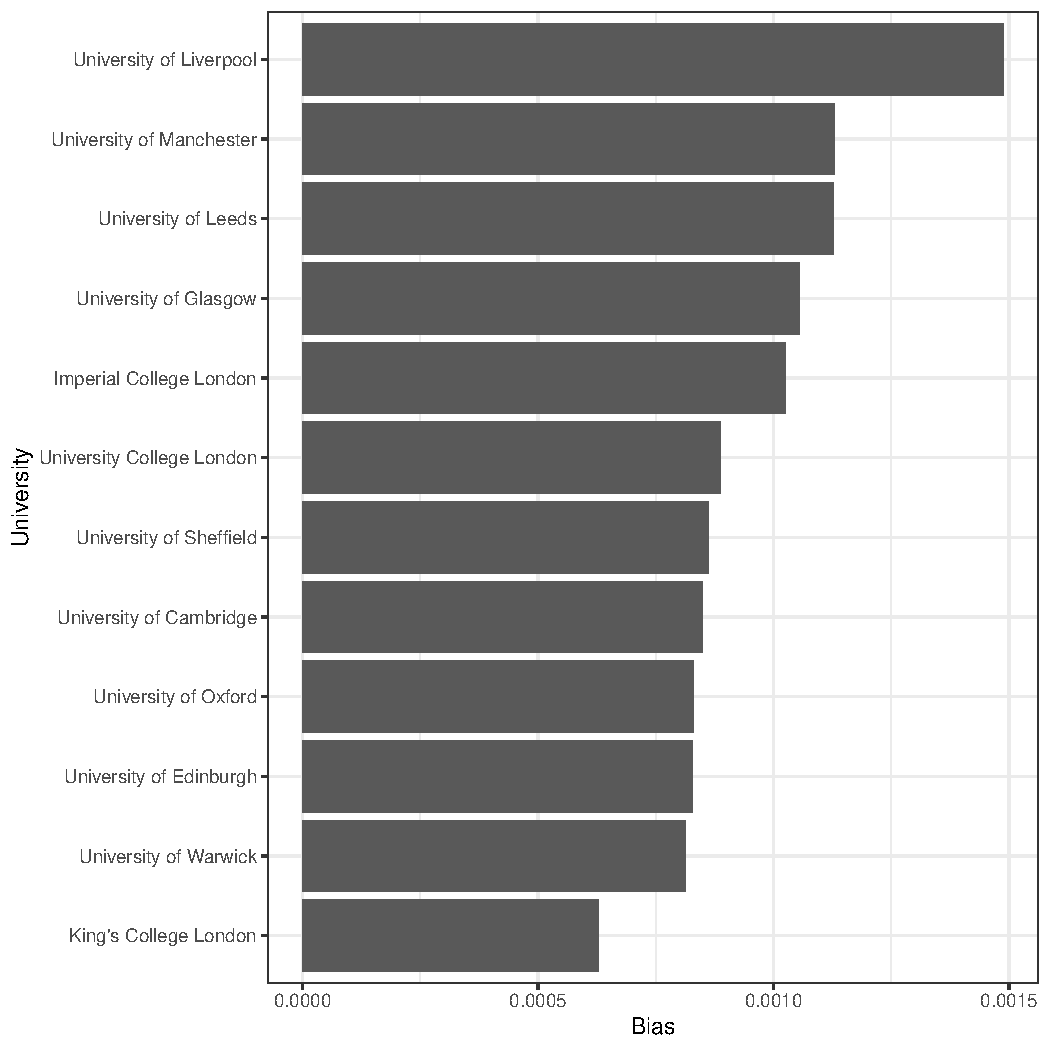
\includegraphics[height=0.7\textheight]{rank_uni.pdf}
	\caption{Similar to the previous comparison across various classifications, this figure shows the ranking of the extent of gender bias in universities. For each university, the total number of funded males or females in all classifications during the period 2015~2022 is summed up, and divided by the total number of HESA male or female staff in the corresponding university. The results are then used to calculate the degree of bias by finding the ratio for males minus the ratio for females in each university.}
\end{figure}

\noindent From the results shown, gender differences can be observed in all the universities we are studying. Among these universities, our results suggest that the gender gap at King's College London and the University of Warwick is comparatively smaller. In contrast, the gap in the other universities shows a baptism pattern with a larger gender gap. The gap is the largest for the results in the University of Liverpool and the University of Manchester compared to other institutions. We may conclude that the institution's ranking might potentially affect gender equality in STEM research funding. Additionally, a sad observation is that from this comparison result, there is no signal of an improving trend of reducing the gap. Though the ratio of funded males in recent years is decreasing, the reduction is also seen for females.

\pagebreak